\documentclass{beamer}
\usepackage[utf8]{inputenc}

\usetheme{Madrid}
\usecolortheme{default}
\usepackage{amsmath,amssymb,amsfonts,amsthm}
\usepackage{txfonts}
\usepackage{tkz-euclide}
\usepackage{listings}
\usepackage{adjustbox}
\usepackage{array}
\usepackage{tabularx}
\usepackage{gvv}
\usepackage{lmodern}
\usepackage{circuitikz}
\usepackage{tikz}
\usepackage{graphicx}
\usepackage{gensymb} 

\setbeamertemplate{page number in head/foot}[totalframenumber]

\usepackage{tcolorbox}
\tcbuselibrary{minted,breakable,xparse,skins}

\definecolor{bg}{gray}{0.95}
\DeclareTCBListing{mintedbox}{O{}m!O{}}{%
breakable=true,
listing engine=minted,
listing only,
minted language=#2,
minted style=default,
minted options={%
linenos,
gobble=0,
breaklines=true,
breakafter=,,
fontsize=\small,
numbersep=8pt,
#1},
boxsep=0pt,
left skip=0pt,
right skip=0pt,
left=25pt,
right=0pt,
top=3pt,
bottom=3pt,
arc=5pt,
leftrule=0pt,
rightrule=0pt,
bottomrule=2pt,
toprule=2pt,
colback=bg,
colframe=orange!70,
enhanced,
overlay={%
\begin{tcbclipinterior}
\fill[orange!20!white] (frame.south west) rectangle ([xshift=20pt]frame.north west);
\end{tcbclipinterior}},
#3,
}
\lstset{
language=C,
basicstyle=\ttfamily\small,
keywordstyle=\color{blue},
stringstyle=\color{orange},
commentstyle=\color{green!60!black},
numbers=left,
numberstyle=\tiny\color{gray},
breaklines=true,
showstringspaces=false,
}

\title{12.264}
\date{October 8, 2025}
\author{EE25BTECH11043 - Nishid Khandagre}

\begin{document}

\frame{\titlepage}

\begin{frame}{Question}
Consider the system of equations
\begin{align*}
2x_1 + x_2 + x_3 &= 0 \\
x_2 - x_3 &= 0 \\
x_1 + x_2 &= 0
\end{align*}
This system has
\begin{itemize}
\item a) a unique solution
\item b) no solution
\item c) infinite number of solutions
\item d) five solutions
\end{itemize}
\end{frame}

\begin{frame}{Solution}
We can represent the system of equations in matrix form as 
\begin{align}
\vec{A}\vec{x} = \vec{0}
\end{align}
\begin{align}
\vec{A} &= \myvec{
2 & 1 & 1 \\
0 & 1 & -1 \\
1 & 1 & 0
}
\end{align}
\begin{align}
\vec{x} &= \myvec{
x_1 \\ x_2 \\ x_3
}
\end{align}
\end{frame}

\begin{frame}{Solution}
Augmented matrix
\begin{align}
\myvec{
2 & 1 & 1 & \vrule & 0 \\
0 & 1 & -1 & \vrule & 0 \\
1 & 1 & 0 & \vrule & 0
}
\end{align}
Apply the operation $R_1 \rightarrow \frac{1}{2}R_1$:
\begin{align}
\myvec{
1 & 0.5 & 0.5 & \vrule & 0 \\
0 & 1 & -1 & \vrule & 0 \\
1 & 1 & 0 & \vrule & 0
}
\end{align}
\end{frame}

\begin{frame}{Solution}
Apply the operation $R_1 \rightarrow \frac{1}{2}R_1$:
\begin{align}
\myvec{
1 & 0.5 & 0.5 & \vrule & 0 \\
0 & 1 & -1 & \vrule & 0 \\
1 & 1 & 0 & \vrule & 0
}
\end{align}
Then $R_3 \rightarrow R_3 - R_1$:
\begin{align}
\myvec{
1 & 0.5 & 0.5 & \vrule & 0 \\
0 & 1 & -1 & \vrule & 0 \\
0 & 0.5 & -0.5 & \vrule & 0
}
\end{align}
\end{frame}

\begin{frame}{Solution}
Perform the operation $R_3 \rightarrow R_3 - 0.5 R_2$:
\begin{align}
\myvec{
1 & 0.5 & 0.5 & \vrule & 0 \\
0 & 1 & -1 & \vrule & 0 \\
0 & 0 & 0 & \vrule & 0
}
\end{align}
\end{frame}

\begin{frame}{Solution}
From the row echelon form, we can write the new system of equations:
\begin{align}
x_1 + 0.5x_2 + 0.5x_3 &= 0 \\
x_2 - x_3 &= 0
\end{align}
From the second equation, we get:
\begin{align}
x_2 = x_3
\end{align}
Substitute $x_2 = x_3$ into the first equation:
\begin{align}
x_1 + 0.5x_2 + 0.5x_2 &= 0 \\
x_1 + x_2 &= 0 \\
x_1 &= -x_2
\end{align}
\end{frame}

\begin{frame}{Solution}
Let $x_2 = t$, where $t$ is any real number.
Then, we have:
\begin{align}
x_3 &= t \\
x_1 &= -t
\end{align}
So, the solution vector is:
\begin{align}
\myvec{x_1 \\ x_2 \\ x_3} = t \myvec{-1 \\ 1 \\ 1}, \quad t \in \mathbb{R}
\end{align}
Since there is one free parameter ($t$), the system has infinitely many solutions. This is also indicated by the rank of matrix A being less than 3 (rank is 2), and the system is consistent (homogeneous systems are always consistent).
Therefore, the answer is option (c).
\end{frame}

\begin{frame}[fragile]
\frametitle{C Code}
\begin{lstlisting}{c}
#include <stdio.h>

// Function to calculate the determinant of a 3x3 matrix
// The matrix is passed as a 1D array in row-major order:
// [a11, a12, a13, a21, a22, a23, a31, a32, a33]
double calculate_determinant_3x3(double* matrix) {
    double det = 0.0;
    
    det = matrix[0] * (matrix[4] * matrix[8] - matrix[5] * matrix[7])
        - matrix[1] * (matrix[3] * matrix[8] - matrix[5] * matrix[6])
        + matrix[2] * (matrix[3] * matrix[7] - matrix[4] * matrix[6]);

    return det;
}
\end{lstlisting}
\end{frame}

\begin{frame}[fragile]
\frametitle{Python Code using Shared C Library}
\begin{lstlisting}{python}
import ctypes
import numpy as np
import matplotlib.pyplot as plt
from mpl_toolkits.mplot3d import Axes3D
from matplotlib.lines import Line2D

# Load the shared library
lib_solver = ctypes.CDLL("./code21.so")

# Define the argument types and return type for the C function
lib_solver.calculate_determinant_3x3.argtypes = [
    ctypes.POINTER(ctypes.c_double)
]
lib_solver.calculate_determinant_3x3.restype = ctypes.c_double
\end{lstlisting}
\end{frame}

\begin{frame}[fragile]
\frametitle{Python Code using Shared C Library}
\begin{lstlisting}{python}
# Define the coefficient matrix for the system of equations:
# Coefficient matrix A:
# [2  1  1]
# [0  1 -1]
# [1  1  0]

coefficient_matrix_np = np.array([
    2.0, 1.0, 1.0,
    0.0, 1.0, -1.0,
    1.0, 1.0, 0.0
], dtype=np.float64)
matrix_reshaped = coefficient_matrix_np.reshape(3,3)
print("Coefficient Matrix:")
print(matrix_reshaped)
# Create a ctypes array from the numpy array for the C function
matrix_c = (ctypes.c_double * len(coefficient_matrix_np))(*coefficient_matrix_np)
\end{lstlisting}
\end{frame}

\begin{frame}[fragile]
\frametitle{Python Code using Shared C Library }
\begin{lstlisting}{python}
# Call the C function to calculate the determinant
determinant = lib_solver.calculate_determinant_3x3(matrix_c)

print(f"\nCalculated Determinant: {determinant:.4f}")

# Determine the nature of the solutions
if abs(determinant) > 1e-9:
    solution_type = "a) a unique solution (trivial solution)"
    plot_title_suffix = "Unique Solution (Intersection at Origin)"
else:
    solution_type = "c) infinite number of solutions"
    plot_title_suffix = "Infinite Solutions (Intersection along a Line)"

print(f"\nFor this homogeneous system, the conclusion is:\n{solution_type}")
\end{lstlisting}
\end{frame}

\begin{frame}[fragile]
\frametitle{Python Code using Shared C Library }
\begin{lstlisting}{python}
# --- 3D Plotting of Planes ---
fig = plt.figure(figsize=(10, 8))
ax = fig.add_subplot(111, projection='3d')
# Define a range for x, y, z
r = 3
x = np.linspace(-r, r, 10)
y = np.linspace(-r, r, 10)
X, Y = np.meshgrid(x, y)

# Equation 1: 2x1 + x2 + x3 = 0  => x3 = -2x1 - x2
Z1 = -2*X - Y
ax.plot_surface(X, Y, Z1, alpha=0.5, color='cyan', label='2x1 + x2 + x3 = 0')

# Equation 2: x2 - x3 = 0  => x3 = x2
Z2 = Y
ax.plot_surface(X, Y, Z2, alpha=0.5, color='magenta', label='x2 - x3 = 0')
\end{lstlisting}
\end{frame}

\begin{frame}[fragile]
\frametitle{Python Code using Shared C Library }
\begin{lstlisting}{python}
# Equation 3: x1 + x2 = 0  => x2 = -x1
X3_plot, Z3_plot = np.meshgrid(x, np.linspace(-r, r, 10))
Y3_plot = -X3_plot
ax.plot_surface(X3_plot, Y3_plot, Z3_plot, alpha=0.5, color='yellow', label='x1 + x2 = 0')

# Find the intersection line: (-t, t, t)
t = np.linspace(-r, r, 100)
intersection_line_x = -t
intersection_line_y = t
intersection_line_z = t
ax.plot(intersection_line_x, intersection_line_y, intersection_line_z,
        color='red', linewidth=3, label='Intersection Line (-t, t, t)')
# Add a point at the origin (trivial solution)
ax.scatter(0, 0, 0, color='red', s=100, label='Origin (0,0,0)', zorder=5)
\end{lstlisting}
\end{frame}

\begin{frame}[fragile]
\frametitle{Python Code using Shared C Library}
\begin{lstlisting}{python}
ax.set_xlabel('x1')
ax.set_ylabel('x2')
ax.set_zlabel('x3')
ax.set_title(f"Planes for System of Equations: {plot_title_suffix}\n(Det = {determinant:.0f})")
custom_lines = [
    Line2D([0], [0], color='cyan', lw=4, alpha=0.5),
    Line2D([0], [0], color='magenta', lw=4, alpha=0.5),
    Line2D([0], [0], color='yellow', lw=4, alpha=0.5),
    Line2D([0], [0], color='red', lw=3)
]
ax.legend(custom_lines,
          ['2x1 + x2 + x3 = 0', 'x2 - x3 = 0', 'x1 + x2 = 0', 'Intersection Line'],
          loc='upper left', bbox_to_anchor=(0.8, 0.95))

plt.tight_layout()
plt.show()
\end{lstlisting}
\end{frame}

\begin{frame}[fragile]
\frametitle{Pure Python Code}
\begin{lstlisting}{python}
import numpy as np
import matplotlib.pyplot as plt
from mpl_toolkits.mplot3d import Axes3D
from matplotlib.lines import Line2D

def calculate_determinant_3x3_python(matrix):
    if matrix.shape != (3, 3):
        raise ValueError("Input matrix must be 3x3.")
    a, b, c = matrix[0, 0], matrix[0, 1], matrix[0, 2]
    d, e, f = matrix[1, 0], matrix[1, 1], matrix[1, 2]
    g, h, i = matrix[2, 0], matrix[2, 1], matrix[2, 2]
    det = a * (e * i - f * h) - b * (d * i - f * g) + c * (d * h - e * g)
    return det
\end{lstlisting}
\end{frame}

\begin{frame}[fragile]
\frametitle{Pure Python Code}
\begin{lstlisting}{python}
coefficient_matrix_np = np.array([
    [2.0, 1.0, 1.0],
    [0.0, 1.0, -1.0],
    [1.0, 1.0, 0.0]
], dtype=np.float64)
print("Coefficient Matrix:")
print(coefficient_matrix_np)
determinant = calculate_determinant_3x3_python(coefficient_matrix_np)
if abs(determinant) > 1e-9:
    solution_type = "a) a unique solution (trivial solution)"
    plot_title_suffix = "Unique Solution (Intersection at Origin)"
    has_intersection_line = False
else:
    solution_type = "c) infinite number of solutions"
    plot_title_suffix = "Infinite Solutions (Intersection along a Line)"
    has_intersection_line = True
\end{lstlisting}
\end{frame}

\begin{frame}[fragile]
\frametitle{Pure Python Code}
\begin{lstlisting}
print(f"\nFor this homogeneous system, the conclusion is:\n{solution_type}")

fig = plt.figure(figsize=(10, 8))
ax = fig.add_subplot(111, projection='3d')

r_range = 3
x_vals = np.linspace(-r_range, r_range, 10)
y_vals = np.linspace(-r_range, r_range, 10)
X, Y = np.meshgrid(x_vals, y_vals)

Z1 = -2*X - Y
ax.plot_surface(X, Y, Z1, alpha=0.5, color='cyan', label='2x1 + x2 + x3 = 0')

Z2 = Y
ax.plot_surface(X, Y, Z2, alpha=0.5, color='magenta', label='x2 - x3 = 0')
\end{lstlisting}
\end{frame}

\begin{frame}[fragile]
\frametitle{Pure Python Code}
\begin{lstlisting}
X3_plot, Z3_plot = np.meshgrid(x_vals, np.linspace(-r_range, r_range, 10))
Y3_plot = -X3_plot
ax.plot_surface(X3_plot, Y3_plot, Z3_plot, alpha=0.5, color='yellow', label='x1 + x2 = 0')

if has_intersection_line:
    t = np.linspace(-r_range, r_range, 100)
    intersection_line_x = -t
    intersection_line_y = t
    intersection_line_z = t
    ax.plot(intersection_line_x, intersection_line_y, intersection_line_z,
            color='red', linewidth=3, label='Intersection Line (-t, t, t)')

ax.scatter(0, 0, 0, color='red', s=100, label='Origin (0,0,0)', zorder=5)
\end{lstlisting}
\end{frame}

\begin{frame}[fragile]
\frametitle{Pure Python Code}
\begin{lstlisting}
ax.set_xlabel('x1')
ax.set_ylabel('x2')
ax.set_zlabel('x3')
ax.set_title(f"Planes for System of Equations")

custom_lines = [
    Line2D([0], [0], color='cyan', lw=4, alpha=0.5),
    Line2D([0], [0], color='magenta', lw=4, alpha=0.5),
    Line2D([0], [0], color='yellow', lw=4, alpha=0.5),
    Line2D([0], [0], color='red', lw=3)
]
ax.legend(custom_lines,
          ['2x1 + x2 + x3 = 0', 'x2 - x3 = 0', 'x1 + x2 = 0', 'Intersection Line'],
          loc='upper left', bbox_to_anchor=(0.8, 0.95))

plt.tight_layout()
plt.show()
\end{lstlisting}
\end{frame}

\begin{frame}{Plot by Python using shared output from C}
\begin{figure}[H]
        \centering
        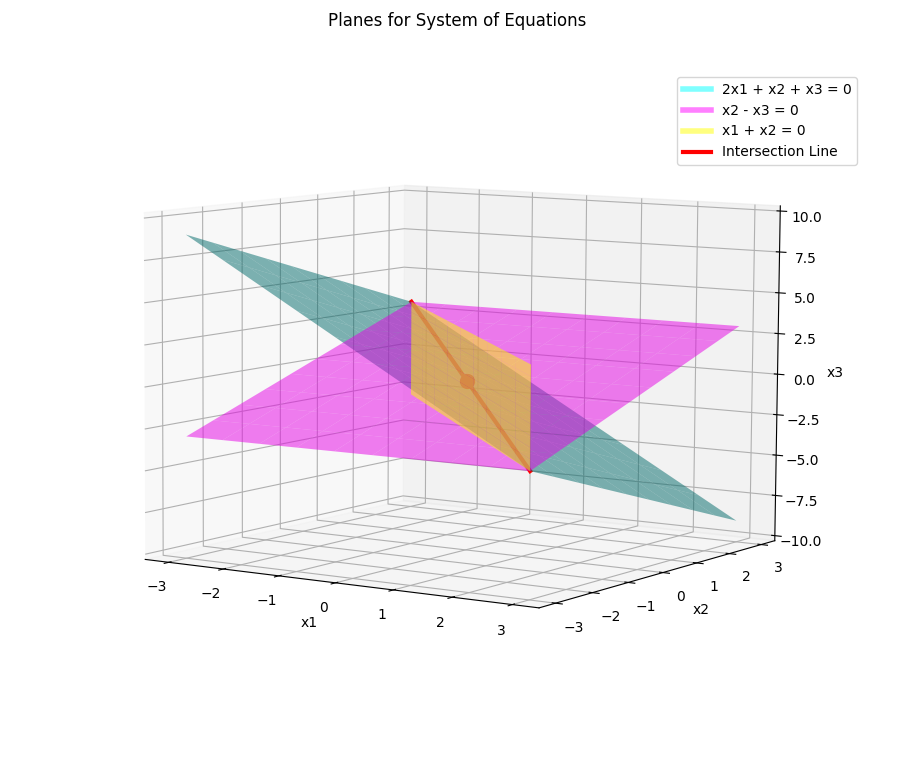
\includegraphics[width=0.8\columnwidth]{../figs/fig1.png}
        \caption{}
        \label{fig:1}
    \end{figure}
\end{frame}

 \begin{frame}{Plot by Python only}
\begin{figure}[H]
        \centering
        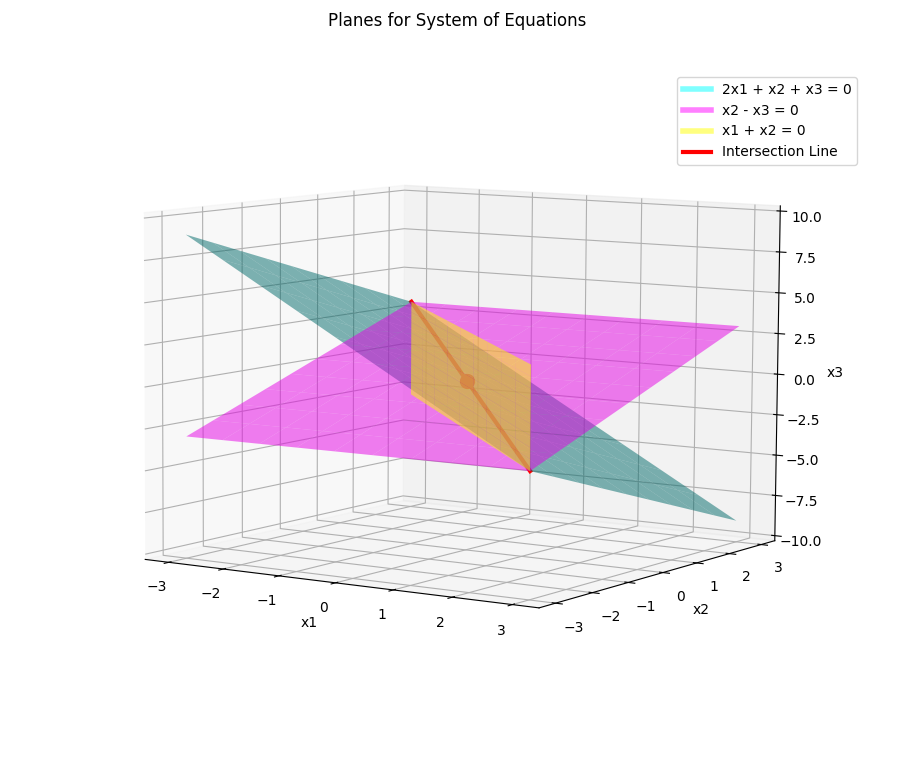
\includegraphics[width=0.8\columnwidth]{../figs/fig2.png}
        \caption{}
        \label{fig:2}
    \end{figure}
\end{frame}

\end{document}
